\chapter{Métodos de Análise de Sincronização de Fase}
\label{chap:6_metodos_de_analise_de_sincronizacao_de_fase}

Neste capítulo, apresentamos os fundamentos teóricos e práticos dos métodos utilizados para analisar a sincronização de fase entre sinais fisiológicos. Em particular, discutiremos o Phase Lag Index (PLI) e o Cross-Frequency Phase Linearity Measurement (CF-PLM). Também foi testado o tradicional Phase Locking Value (PLV) para comparação e os resultados obtidos com o PLV estão disponíveis no anexo para referência. Para este estudo, optamos por utilizar o PLI para a sincronização entre canais de EEG (same-frequency) e o CF-PLM para a análise entre EEG e ECG (cross-frequency).

\section{Fundamentos dos Métodos}

A análise de sincronização de fase visa quantificar a consistência da diferença de fase entre dois sinais ao longo do tempo. Os métodos utilizados neste estudo são baseados em abordagens que extraem a fase instantânea dos sinais por meio da Transformada de Hilbert, permitindo a análise de como as fases se relacionam entre si.

\subsection{Phase Lag Index (PLI)}

O PLI é um índice amplamente utilizado para medir a sincronização de fase entre sinais que operam na mesma faixa de frequência, como os canais de EEG dentro de uma mesma banda. Ao contrário do Phase Locking Value (PLV), o PLI é robusto à mistura de sinais e aos efeitos de condução de volume, pois foca na assimetria da distribuição das diferenças de fase. Especificamente, ele desconsidera valores próximos de zero que podem resultar de sincronizações espúrias, muitas vezes induzidas por fontes comuns ou artefatos, concentrando-se apenas em atrasos de fase que são mais informativos sobre a interação funcional.

Conforme discutido por \citeauthor{seraj2018cerebral} (\citeyear{seraj2018cerebral}), o PLI apresenta vantagens metodológicas, fornecendo uma medida mais pura da sincronização de fase, uma vez que elimina a influência de picos que podem ocorrer devido a volume conduction ou outras fontes de ruído. Essa robustez torna o PLI particularmente adequado para a avaliação da sincronização entre canais de EEG, onde a variabilidade e a interferência de sinais de fundo podem comprometer a precisão de medidas tradicionais como o PLV.

Além disso, o PLI é eficaz na detecção de atrasos sistemáticos entre os sinais, contribuindo para uma melhor compreensão da dinâmica funcional cerebral. No entanto, vale ressaltar que, para interações entre sinais que operam em frequências distintas (por exemplo, entre EEG e ECG), métodos como o CF-PLM são mais indicados. Nesta pesquisa, optamos por utilizar o PLI para a análise de sincronização entre canais de EEG em bandas idênticas, enquanto empregamos o CF-PLM para investigar a sincronização cross-frequency entre EEG e ECG. Os resultados comparativos obtidos com o PLV também foram testados e estão disponíveis no anexo para referência.

\subsection{Cross-Frequency Phase Linearity Measurement (CF-PLM)}

O CF-PLM é um método desenvolvido para analisar a sincronização de fase entre sinais que operam em frequências distintas, ou seja, para detectar acoplamento cross-frequency. Essa abordagem é especialmente útil para avaliar a relação entre os ritmos neurais do EEG (tipicamente de alta frequência) e o ritmo cardíaco do ECG (geralmente de baixa frequência). 

De acordo com \citeauthor{sorrentino2022detection} (\citeyear{sorrentino2022detection}), o método estende o conceito de Phase Linearity Measurement (PLM) para a análise de n:m sincronização entre sinais, sem a necessidade de hipóteses a priori sobre as frequências envolvidas. O procedimento baseia-se nos seguintes passos:

\begin{enumerate}
    \item \textbf{Cálculo dos Sinais Analíticos:} Para os sinais de interesse \(x(t)\) e \(y(t)\), obtém-se suas representações analíticas \(x_{\mathrm{an}}(t)\) e \(y_{\mathrm{an}}(t)\) por meio da Transformada de Hilbert, que fornecem, respectivamente, as fases \(\phi_x(t)\) e \(\phi_y(t)\).
    \item \textbf{Construção do Sinal Interferométrico:} Calcula-se o sinal interferométrico \(z(t)\) utilizando a fórmula:
    \[
    z(t) = \frac{x_{\mathrm{an}}(t)\, y_{\mathrm{an}}^*(t)}{\lvert x_{\mathrm{an}}(t)\rvert\, \lvert y_{\mathrm{an}}(t)\rvert} = e^{i\Delta \phi(t)},
    \]
    onde \(\Delta \phi(t) = \phi_x(t) - \phi_y(t)\) é a diferença de fase instantânea entre os sinais. Note que \(z(t)\) possui amplitude unitária, isolando assim a informação de fase.
    \item \textbf{Análise da Densidade Espectral de Potência (PSD):} Através da Transformada de Fourier, calcula-se a PSD de \(z(t)\). Em condições de acoplamento iso-frequencial, o pico na PSD é centralizado em \(f = 0\). Já em condições de acoplamento cross-frequency, a presença de um desvio (i.e., um pico deslocado de zero) indica a diferença entre as frequências centrais dos sinais.
    \item \textbf{Cálculo do CF-PLM:} O índice CF-PLM é obtido integrando a PSD em uma janela estreita \([f_\Delta - B, f_\Delta + B]\) centrada no pico (onde \(f_\Delta\) representa a diferença de frequência entre os sinais) e normalizando pelo poder total da PSD:
    \[
    \text{CF-PLM} = \frac{\displaystyle\int_{f_\Delta - B}^{f_\Delta + B} SZ(f) \, df}{\displaystyle\int_{-\infty}^{+\infty} SZ(f) \, df}.
    \]
\end{enumerate}

A transformação do ECG em uma representação senoidal (conforme descrito no Capítulo~\ref{chap:preprocessamento_de_dados}) é crucial para que a extração da fase seja clara e contínua, o que, por sua vez, melhora a detecção de sincronização cross-frequency entre os sinais de EEG e ECG. Essa abordagem permite que o CF-PLM capture com precisão a intensidade do acoplamento, sem que a amplitude dos sinais influencie o índice, tornando-o robusto à variabilidade dos dados.

Em resumo, o CF-PLM possibilita uma estimativa confiável da sincronização de fase entre sinais de frequências diferentes, sendo particularmente indicado para a análise de interações entre os ritmos neurais e o ritmo cardíaco, conforme validado por \citeauthor{sorrentino2022detection} (\citeyear{sorrentino2022detection}).

\subsection{Comparação com o Phase Locking Value (PLV)}

Para fins de validação e comparação, também testamos o PLV, um método tradicional e amplamente utilizado para a análise de sincronização de fase. Conforme destacado por \citeauthor{seraj2018cerebral} (\citeyear{seraj2018cerebral}), embora o PLV seja intuitivo e eficaz na medição da consistência da diferença de fase entre sinais na mesma faixa de frequência, ele apresenta limitações notáveis, como a sua sensibilidade a ruídos e aos efeitos de volume conduction, que podem levar à detecção de sincronizações espúrias.

Essas limitações se tornam ainda mais evidentes na análise cross-frequency, onde os sinais operam em escalas de frequência distintas. Em nossa investigação, os resultados obtidos com o PLV foram utilizados para contrastar a sensibilidade e a robustez dos métodos alternativos: o PLI, para sincronização iso-frequencial entre canais de EEG, e o CF-PLM, para a análise de acoplamento cross-frequency entre EEG e ECG. Os resultados experimentais confirmaram que, embora o PLV seja adequado para sinais com a mesma faixa de frequência, ele não captura de maneira confiável a sincronização entre sinais de diferentes frequências, corroborando as observações de Seraj (2018).

Portanto, optamos por utilizar o PLI e o CF-PLM como índices principais neste estudo. Detalhes comparativos e resultados do PLV, que evidenciam suas limitações e complementam nossa análise, estão disponíveis no anexo.

\section{Validação Experimental com Injeção de Sinais}

Para validar os métodos utilizados neste estudo, realizamos experimentos com injeção controlada de sinais senoidais sobre dados reais de ECG e EEG, adquiridos durante sessões experimentais reais. O objetivo foi verificar a capacidade dos índices CF-PLM, PLV e PLI em identificar corretamente diferentes tipos e intensidades de sincronização de fase artificialmente introduzidas.

A técnica empregada consistiu nas seguintes etapas:

\begin{enumerate}
    \item Seleção de segmentos representativos dos sinais originais de ECG e EEG.
    \item Geração de sinais senoidais com frequências e fases específicas utilizando o modelo de Kuramoto, permitindo controle preciso das condições experimentais.
    \item Aplicação controlada desses sinais sobre os sinais originais usando máscaras de injeção, variando a porcentagem de contribuição (0\%, 25\%, 50\%, 75\%, e 100\%) dos sinais injetados.
    \item Cálculo dos índices CF-PLM, PLV e PLI sobre esses sinais modificados, para avaliar o desempenho dos métodos de sincronização propostos em diferentes cenários.
\end{enumerate}

Foram conduzidos três cenários principais:

\begin{itemize}
    \item \textbf{Cross-frequency (1~Hz no ECG, 40~Hz no EEG):} Para testar especialmente o índice CF-PLM em situações onde o acoplamento ocorre entre frequências distintas.
    \item \textbf{Same-frequency (10~Hz no ECG e EEG com defasagem):} Para avaliar sensibilidade e desempenho de todos os índices quando os sinais apresentam frequências iguais, porém com defasagem de fase fixa configurada (\(\pi/4\)).
    \item \textbf{Same-frequency com phase lag zero (ambos 10~Hz sem defasagem):} Cenário idealizado para demonstrar a robustez do PLI contra sincronização espúria.
\end{itemize}

Exemplos dos sinais antes e após a injeção no cenário Cross-frequency são mostrados nas Figuras~\ref{fig:ecg_injection} e~\ref{fig:eeg_injection}, ilustrando a adição de sinais artificiais em frequências distintas sobre o sinal original.

\begin{figure}[htb]
    \centering
    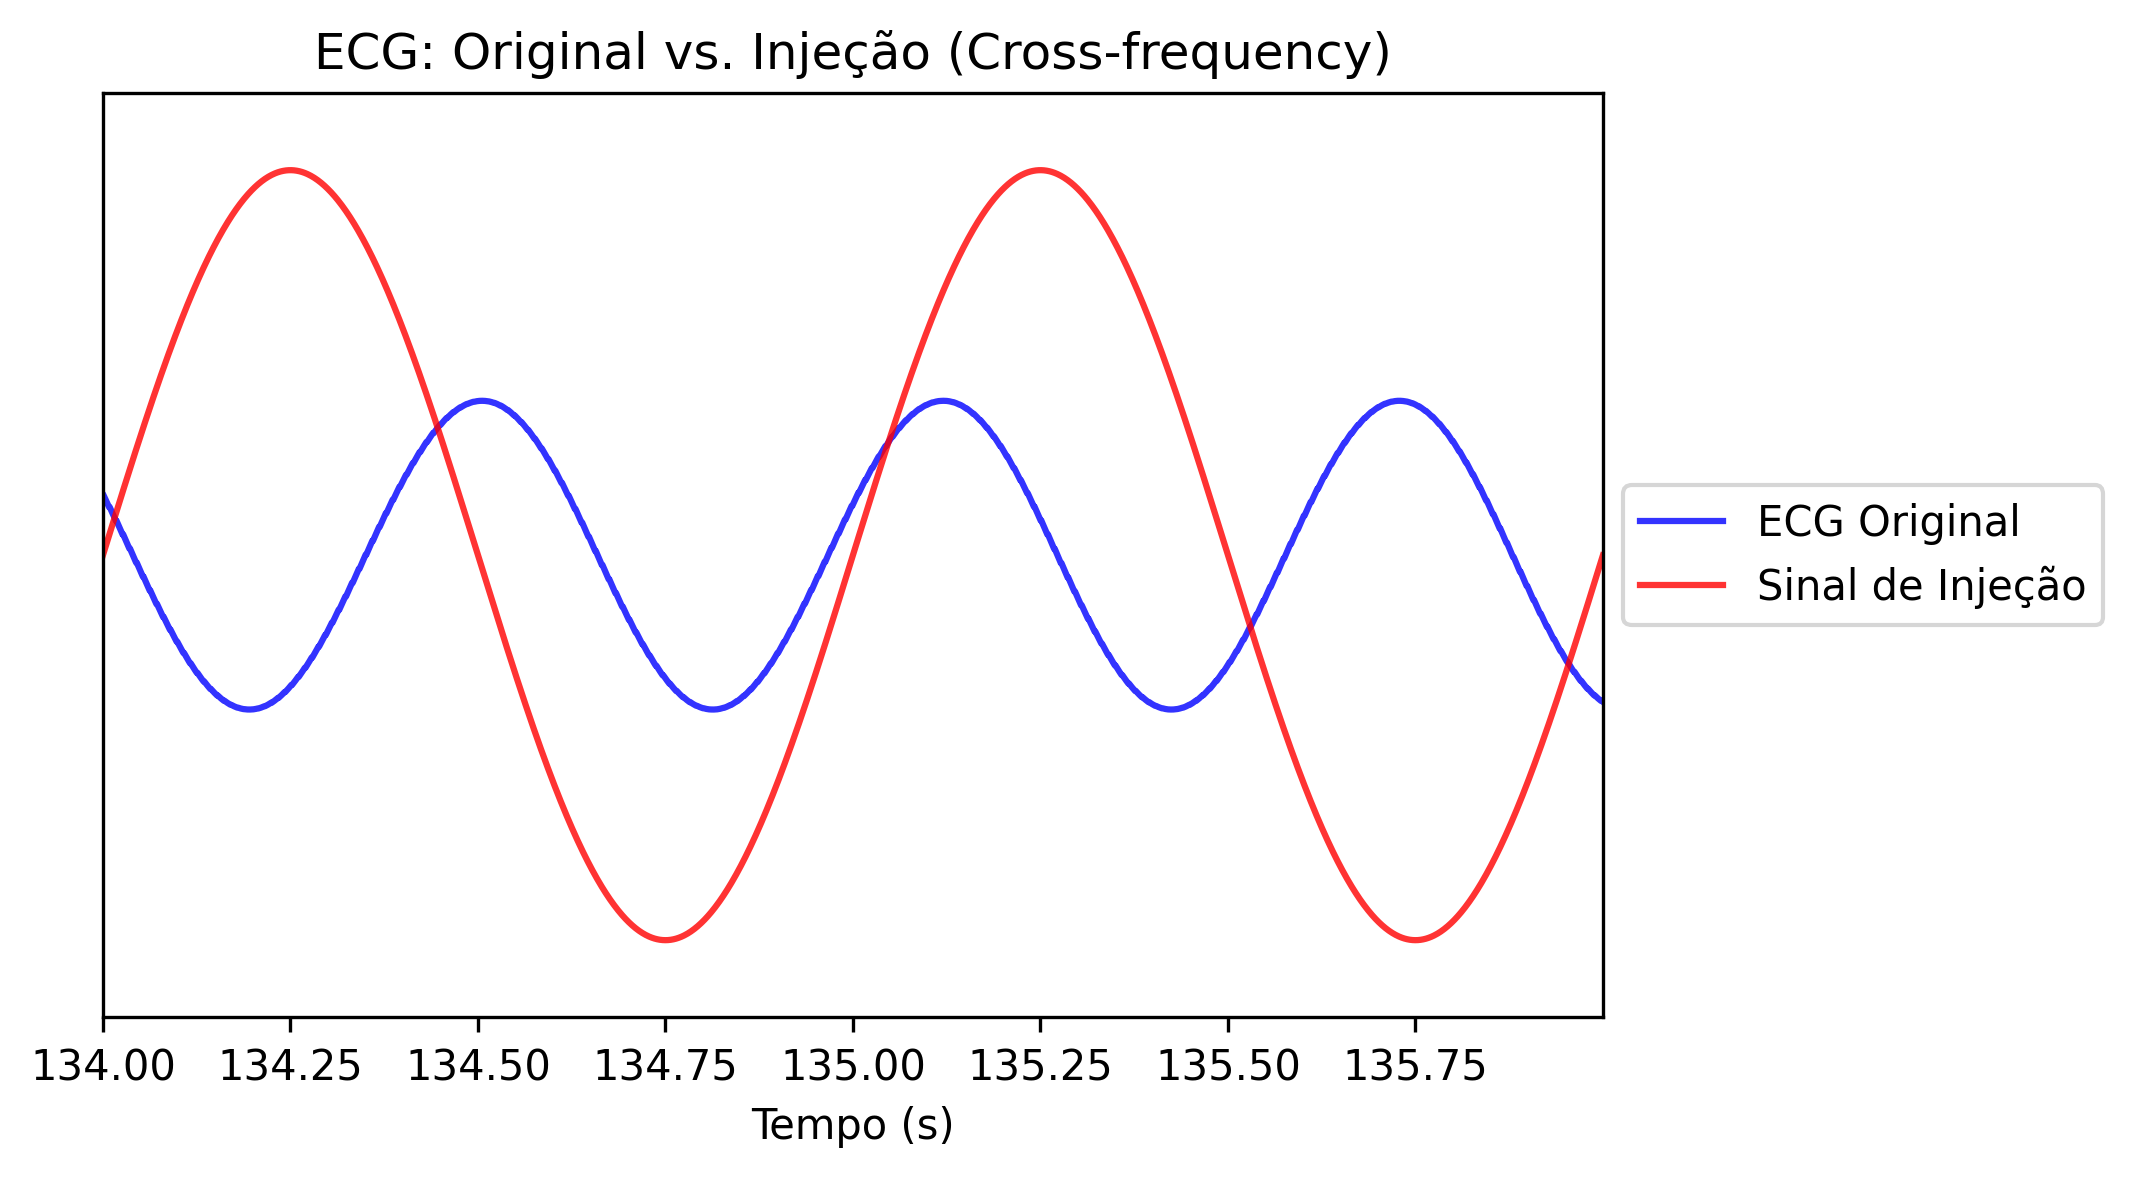
\includegraphics[width=0.8\textwidth]{figs/3_2_testing_connectivity_metrics/1_ECG_Original_vs_Injecao_Cross-frequency.png}
    \caption{ECG: comparação entre o sinal original e o sinal senoidal injetado (1~Hz), cenário Cross-frequency.}
    \label{fig:ecg_injection}
\end{figure}

\begin{figure}[htb]
    \centering
    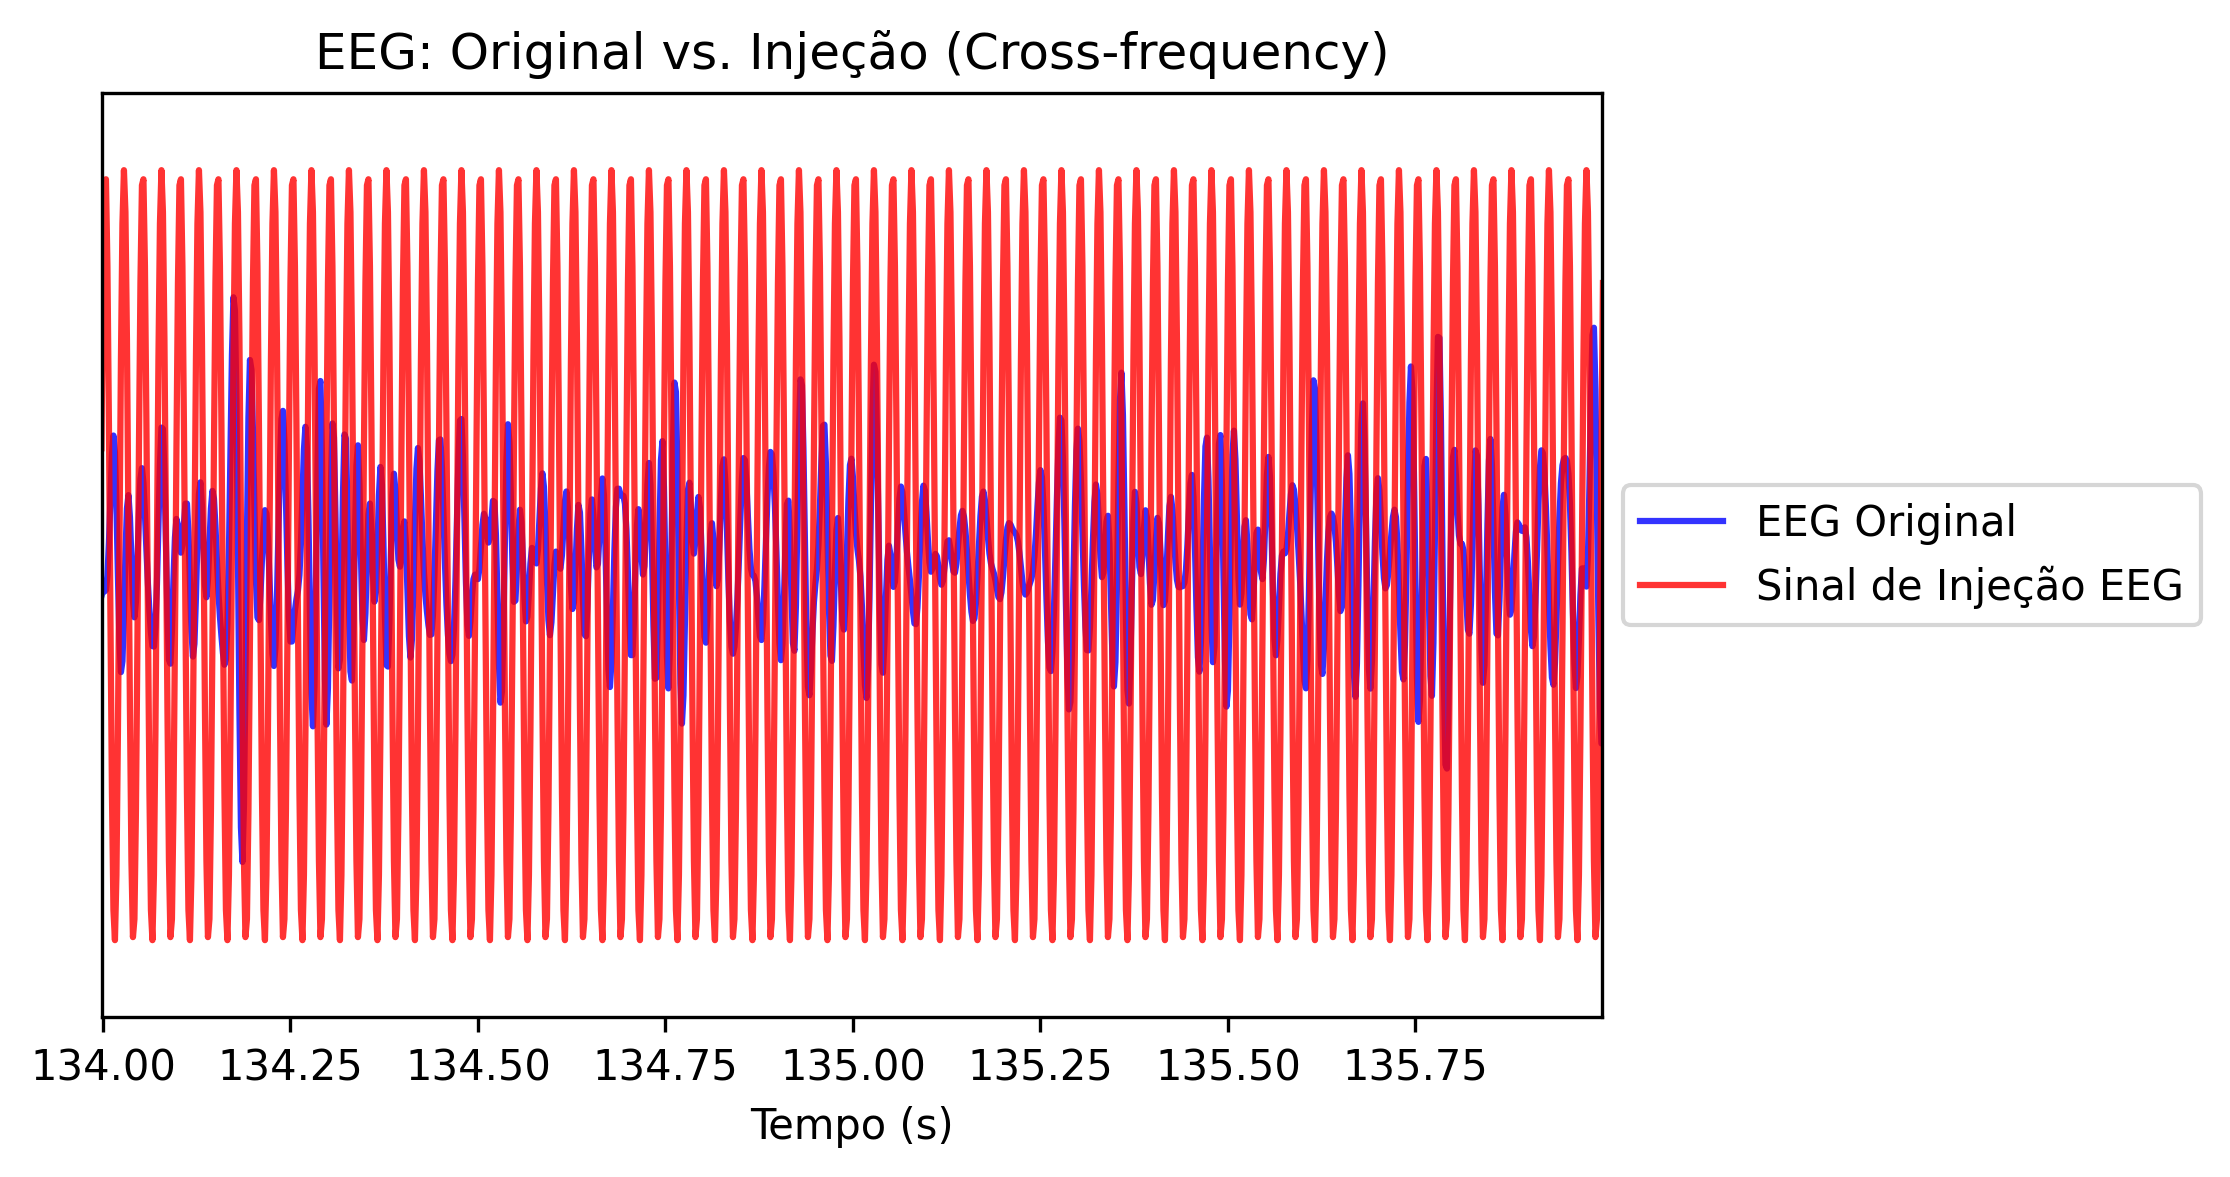
\includegraphics[width=0.8\textwidth]{figs/3_2_testing_connectivity_metrics/3_EEG_Original_vs_Injecao_Cross-frequency.png}
    \caption{EEG: comparação entre o sinal original e o sinal senoidal injetado (40~Hz), cenário Cross-frequency.}
    \label{fig:eeg_injection}
\end{figure}

Já no cenário Same-frequency, onde tanto o ECG quanto o EEG recebem sinais senoidais da mesma frequência (10~Hz) mas com pequena defasagem (\(\pi/4\)), temos os resultados ilustrados pelas Figuras~\ref{fig:eeg_original_vs_injection_samefreq} e~\ref{fig:eeg_injected_samefreq}. Esses gráficos destacam visualmente a interferência resultante da injeção.

\begin{figure}[htb]
    \centering
    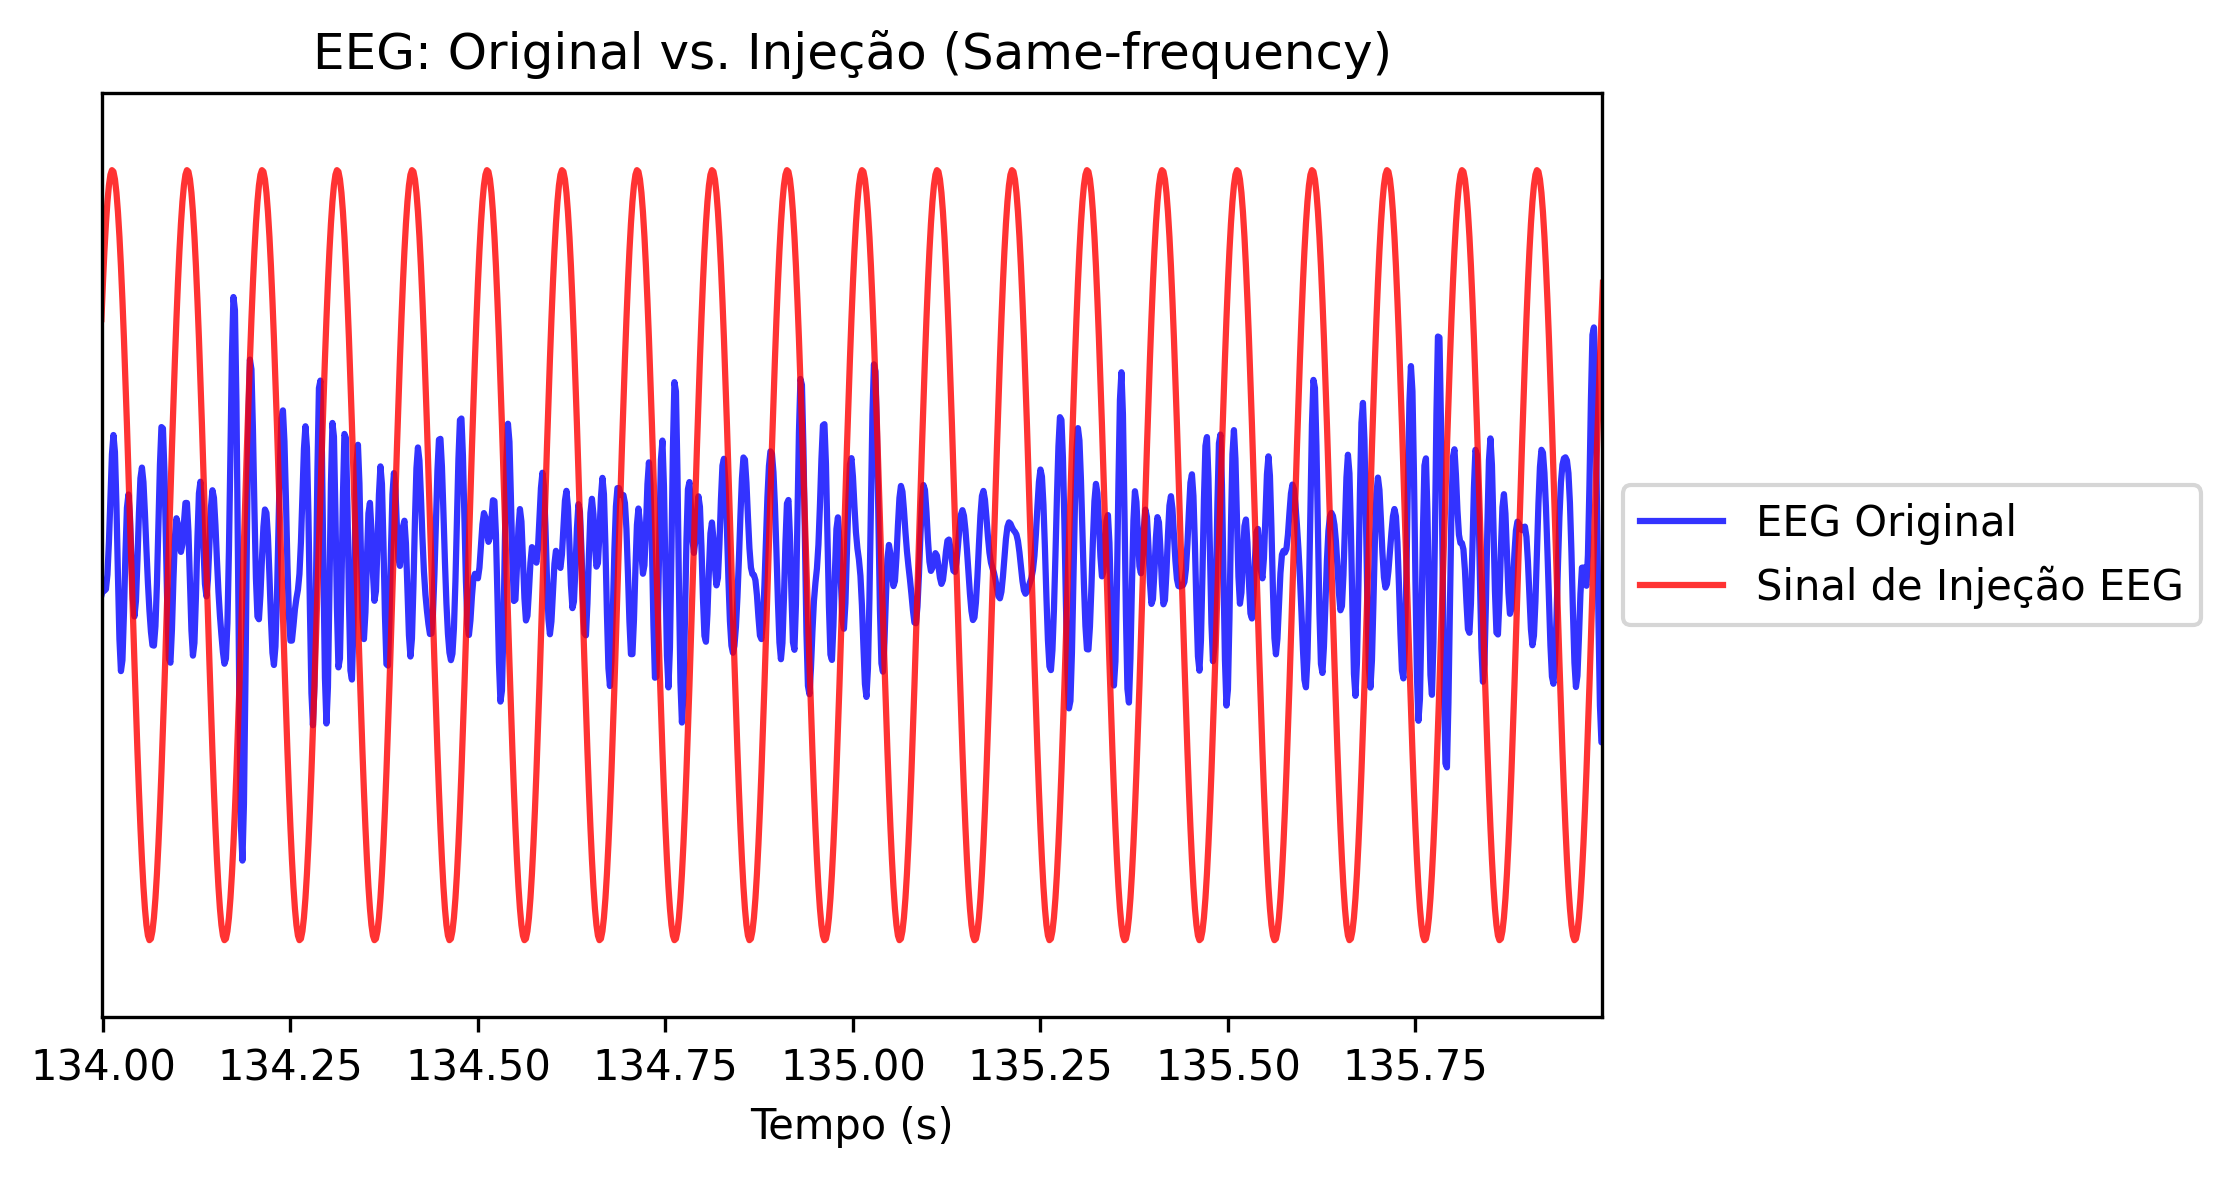
\includegraphics[width=0.8\textwidth]{figs/3_2_testing_connectivity_metrics/10_EEG_Original_vs_Injecao_Same-frequency.png}
    \caption{EEG original (azul) e sinal de injeção de 10 Hz (vermelho) com pequena defasagem (\(\pi/4\)).}
    \label{fig:eeg_original_vs_injection_samefreq}
\end{figure}

\begin{figure}[htb]
    \centering
    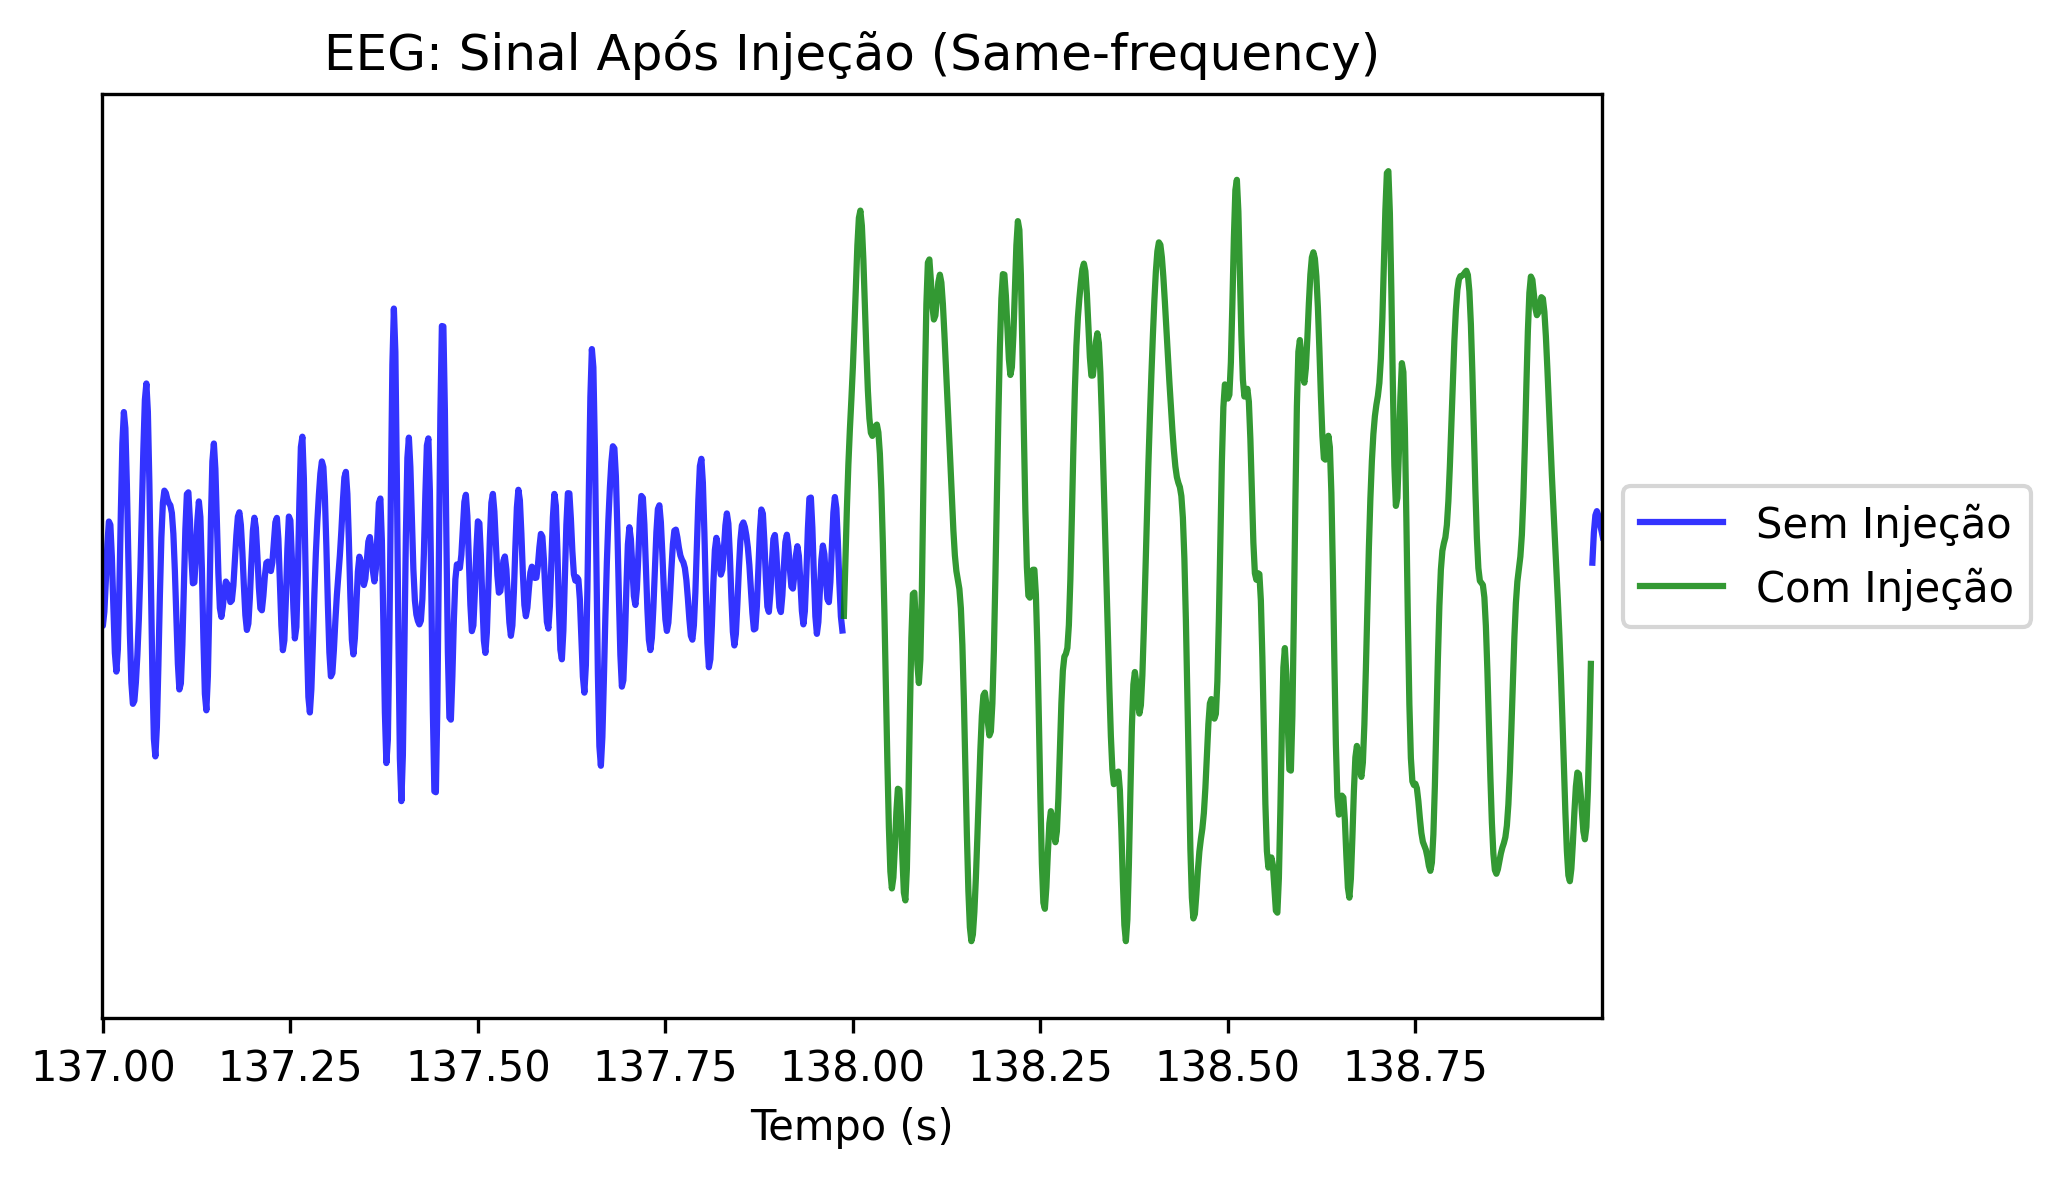
\includegraphics[width=0.8\textwidth]{figs/3_2_testing_connectivity_metrics/11_EEG_Injetado_Same-frequency.png}
    \caption{Sinal de EEG após a injeção controlada de uma senóide (verde) comparado ao sinal original sem injeção (azul).}
    \label{fig:eeg_injected_samefreq}
\end{figure}

Em seguida, realizamos a extração das fases instantâneas usando a transformada de Hilbert e geramos o sinal interferométrico. Esses passos estão exemplificados visualmente nas Figuras~\ref{fig:fases_instantaneas_samefreq} e~\ref{fig:sinal_interferometrico_samefreq}.

\begin{figure}[htb]
    \centering
    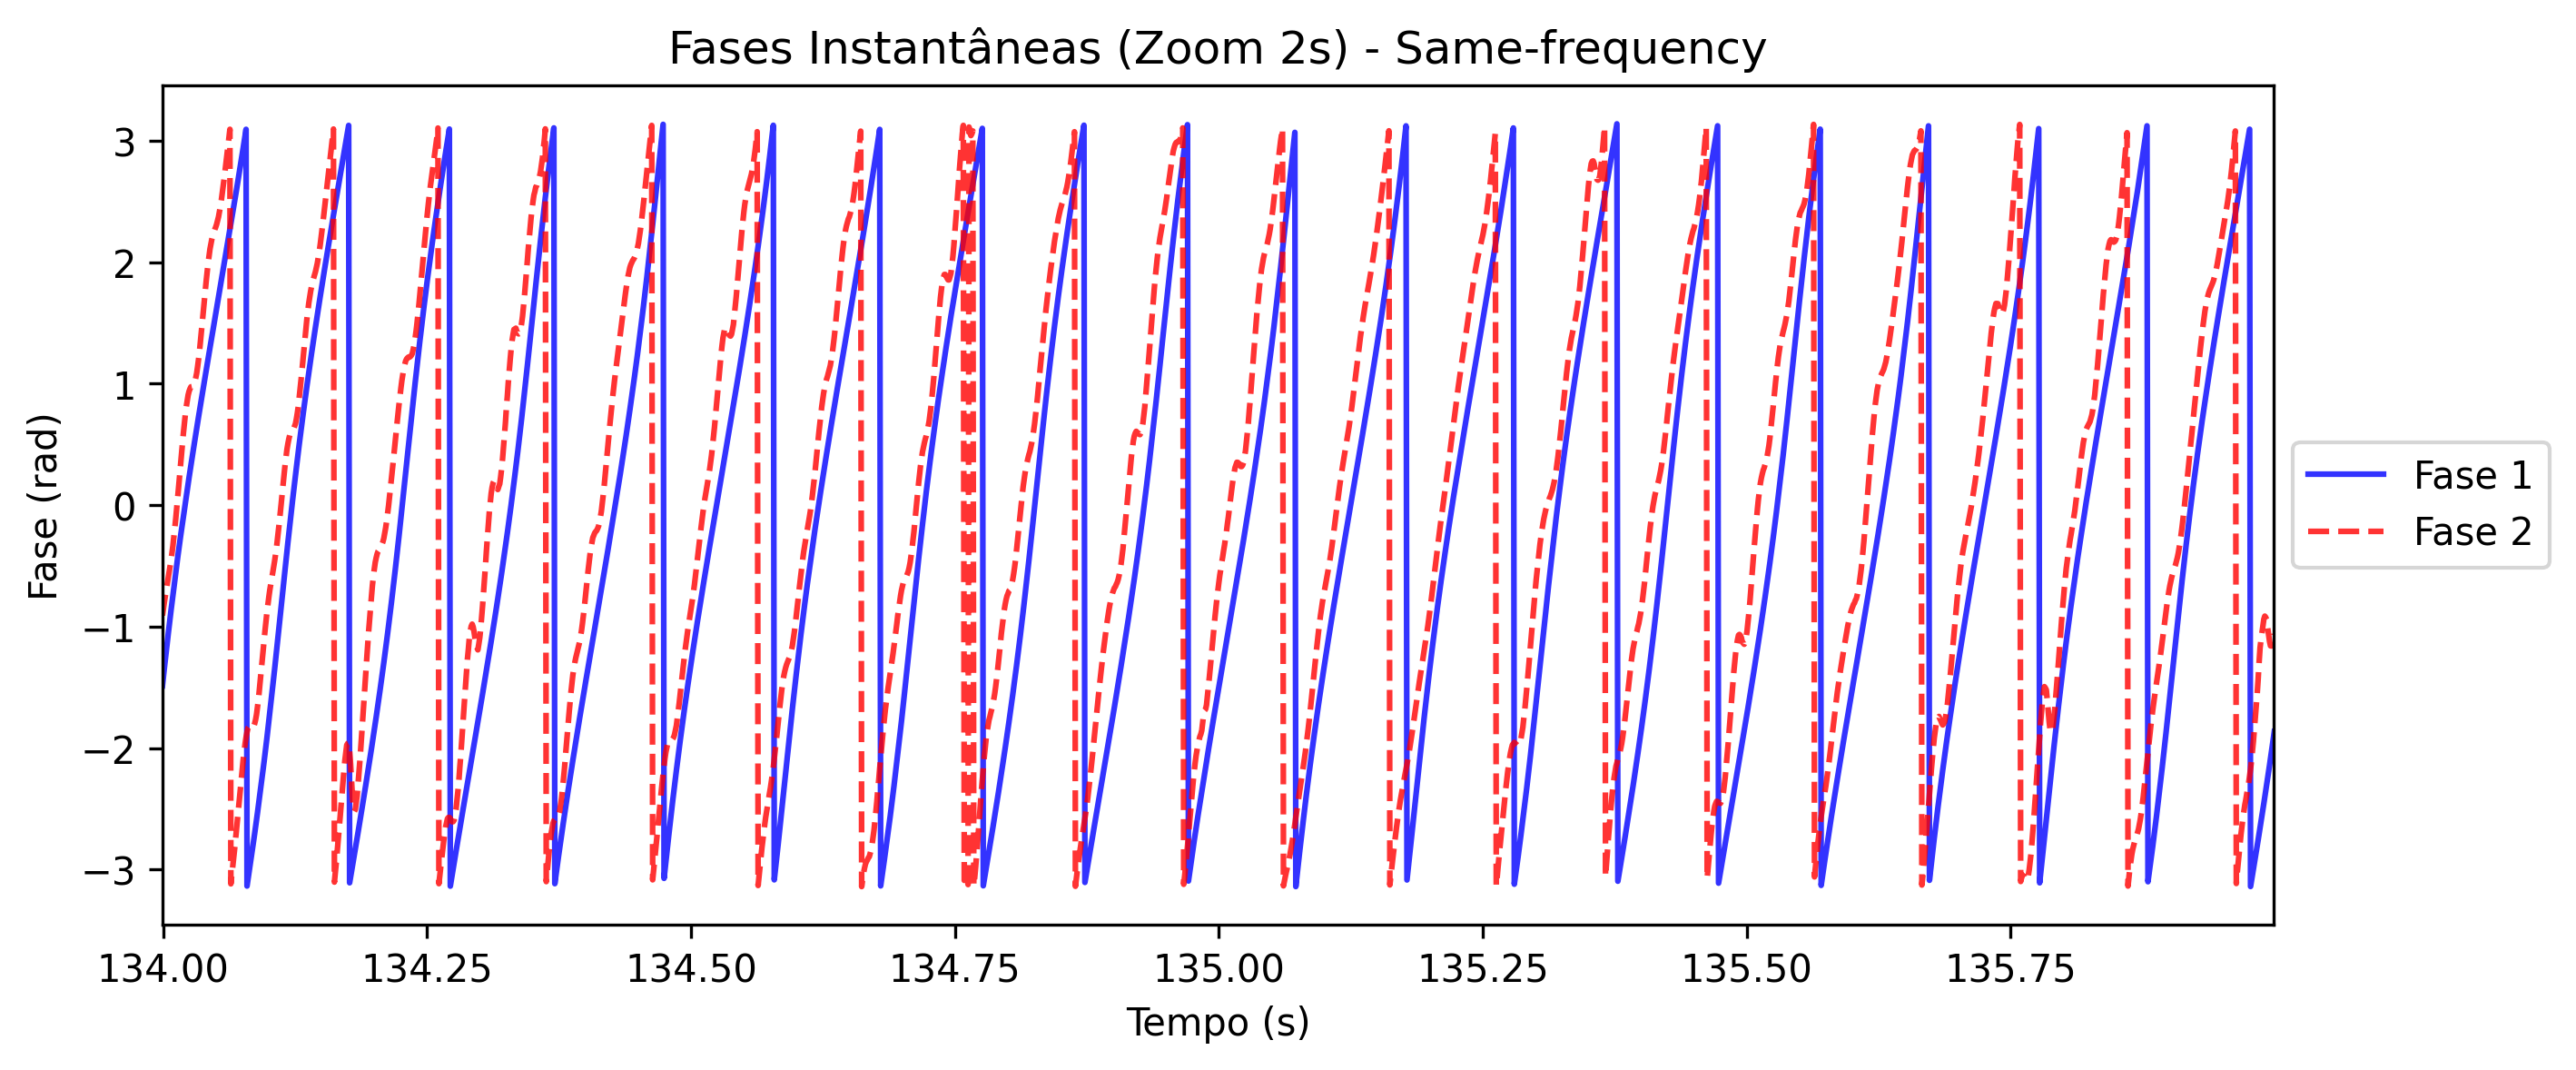
\includegraphics[width=0.8\textwidth]{figs/3_2_testing_connectivity_metrics/12_Passo1_Fases_Same-frequency.png}
    \caption{Fases instantâneas extraídas dos sinais EEG e ECG injetados (ambos a 10 Hz).}
    \label{fig:fases_instantaneas_samefreq}
\end{figure}

\begin{figure}[htb]
    \centering
    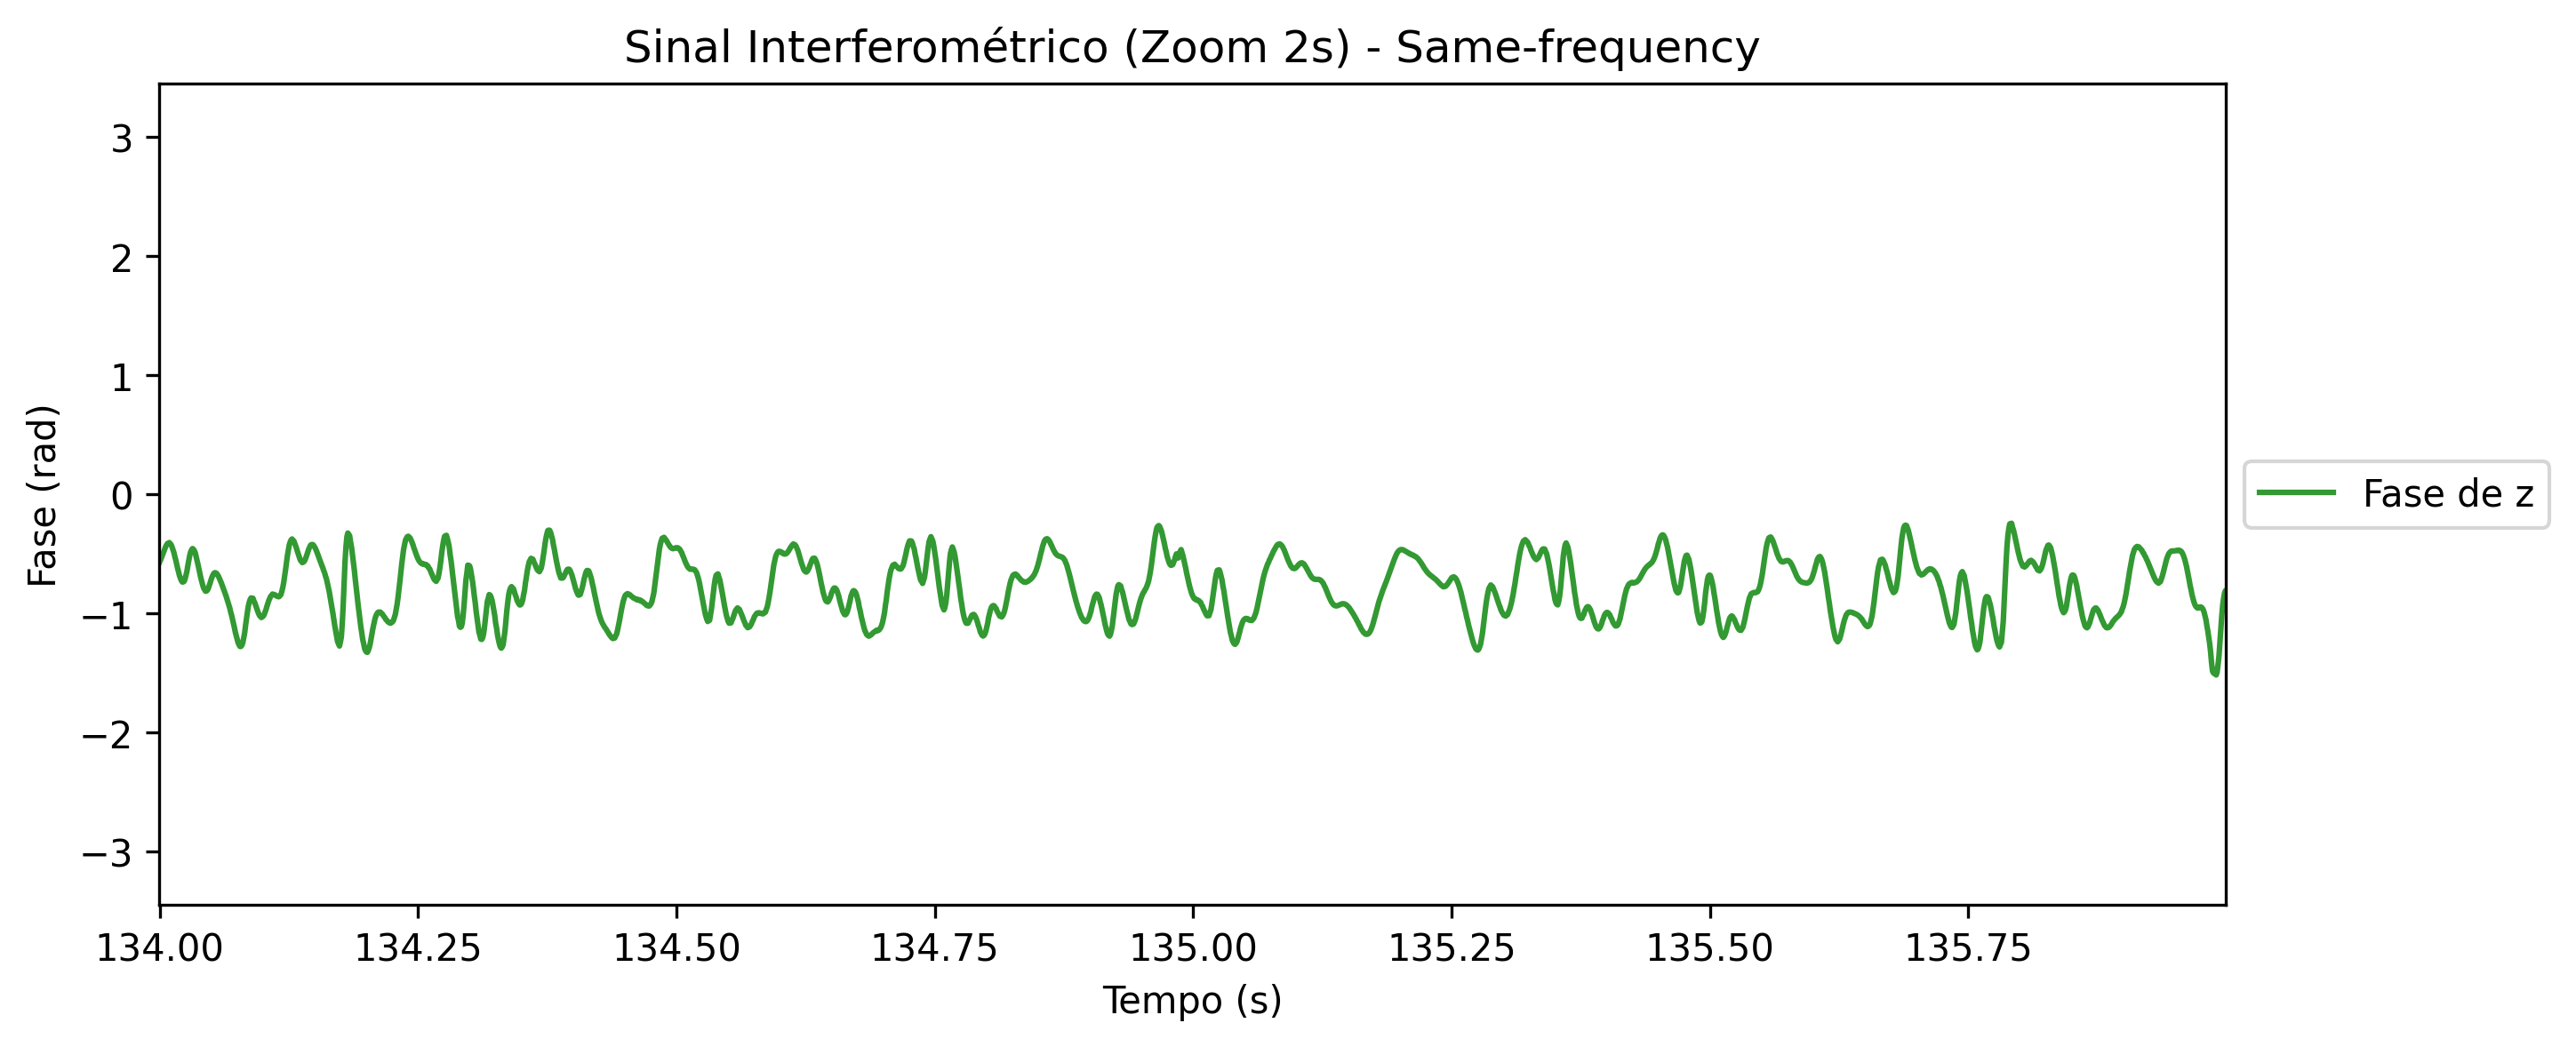
\includegraphics[width=0.8\textwidth]{figs/3_2_testing_connectivity_metrics/13_Passo2_Interferometrico_Same-frequency.png}
    \caption{Sinal interferométrico gerado pela diferença de fase instantânea (cenário same-frequency).}
    \label{fig:sinal_interferometrico_samefreq}
\end{figure}

A seguir, calculamos o índice CF-PLM utilizando a FFT sobre o sinal interferométrico, exemplificado pela Figura~\ref{fig:fft_psd_samefreq}.

\begin{figure}[htb]
    \centering
    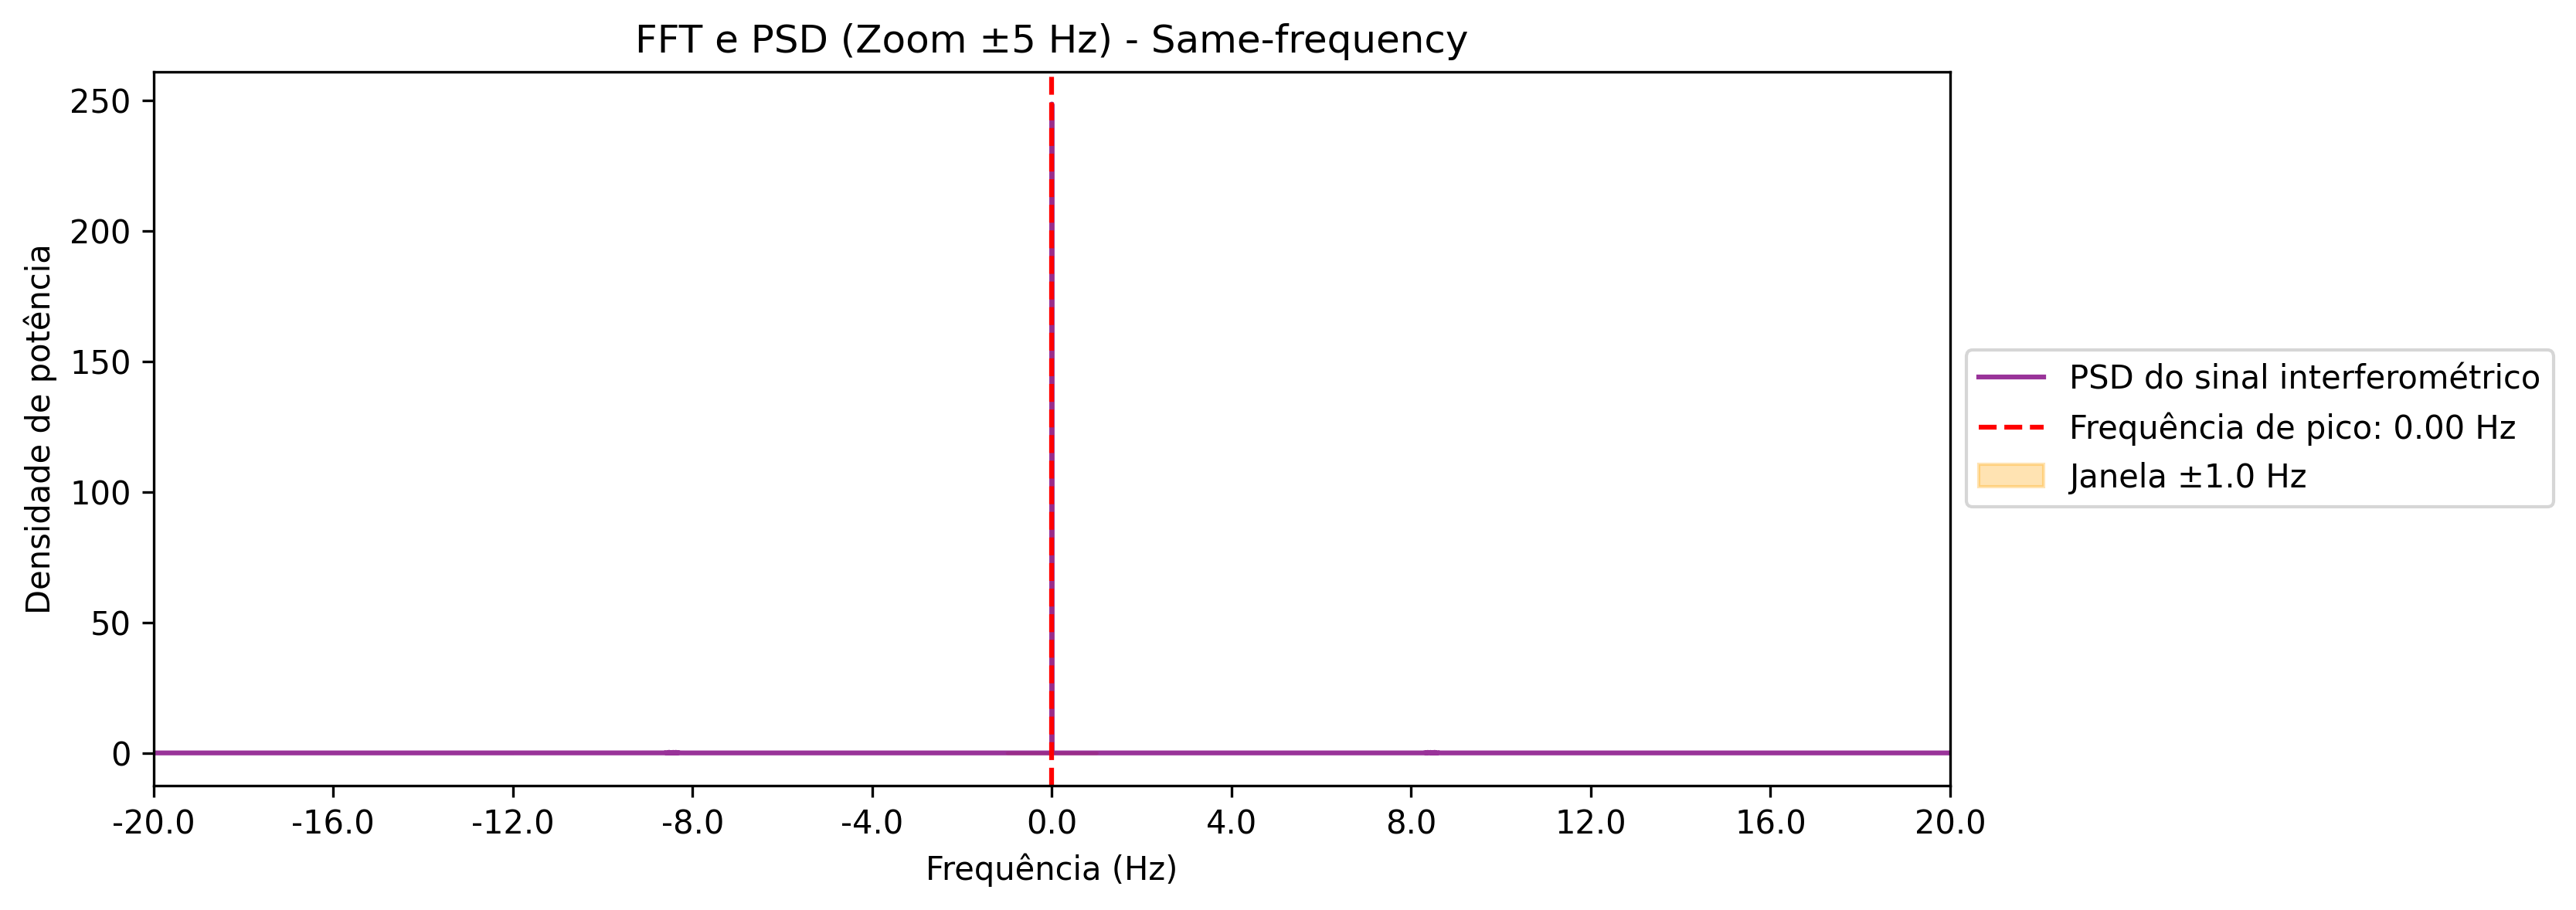
\includegraphics[width=0.8\textwidth]{figs/3_2_testing_connectivity_metrics/14_Passo3_FFT_PSD_Same-frequency.png}
    \caption{PSD do sinal interferométrico, indicando o pico em 0 Hz devido ao offset constante de fase entre os sinais de mesma frequência.}
    \label{fig:fft_psd_samefreq}
\end{figure}

Finalmente, analisamos o cenário especial "Same-frequency Com Phase Lag Zero", onde as fases são perfeitamente sincronizadas. As Figuras~\ref{fig:zerolag_phases_final} e~\ref{fig:zerolag_difference_final} comprovam que o PLI é efetivamente insensível a tais sincronizações.

\begin{figure}[htb]
    \centering
    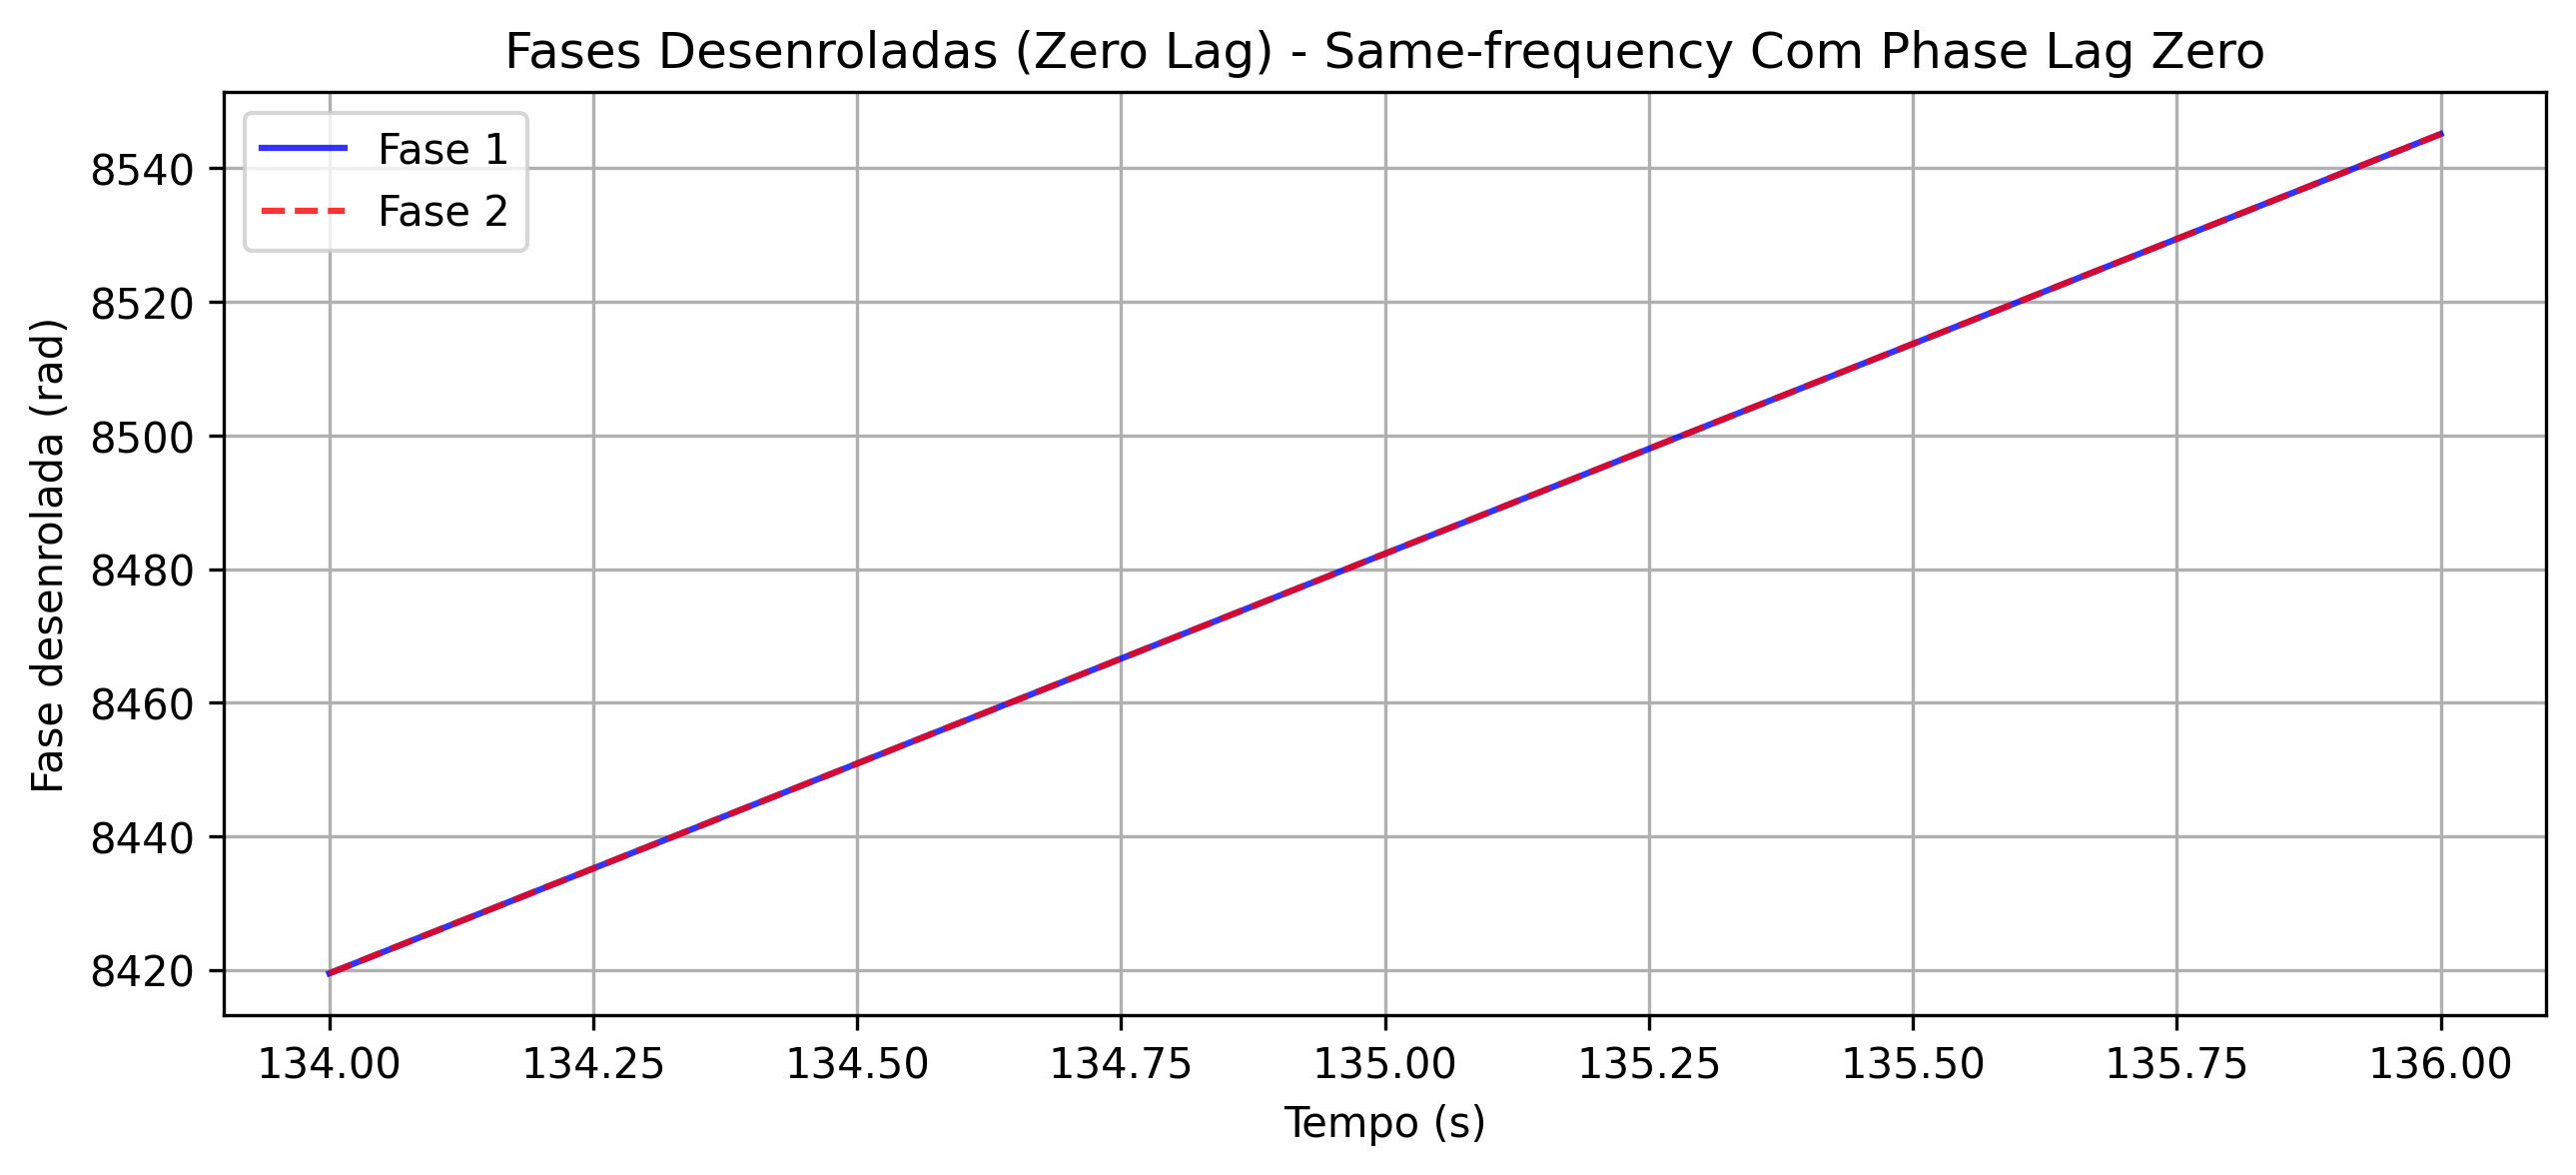
\includegraphics[width=0.8\textwidth]{figs/3_2_testing_connectivity_metrics/15_ZeroLag_Fases_Same-frequency Com Phase Lag Zero.png}
    \caption{Fases desenroladas em cenário sem defasagem (10 Hz), com sobreposição quase exata dos sinais.}
    \label{fig:zerolag_phases_final}
\end{figure}

\begin{figure}[htb]
    \centering
    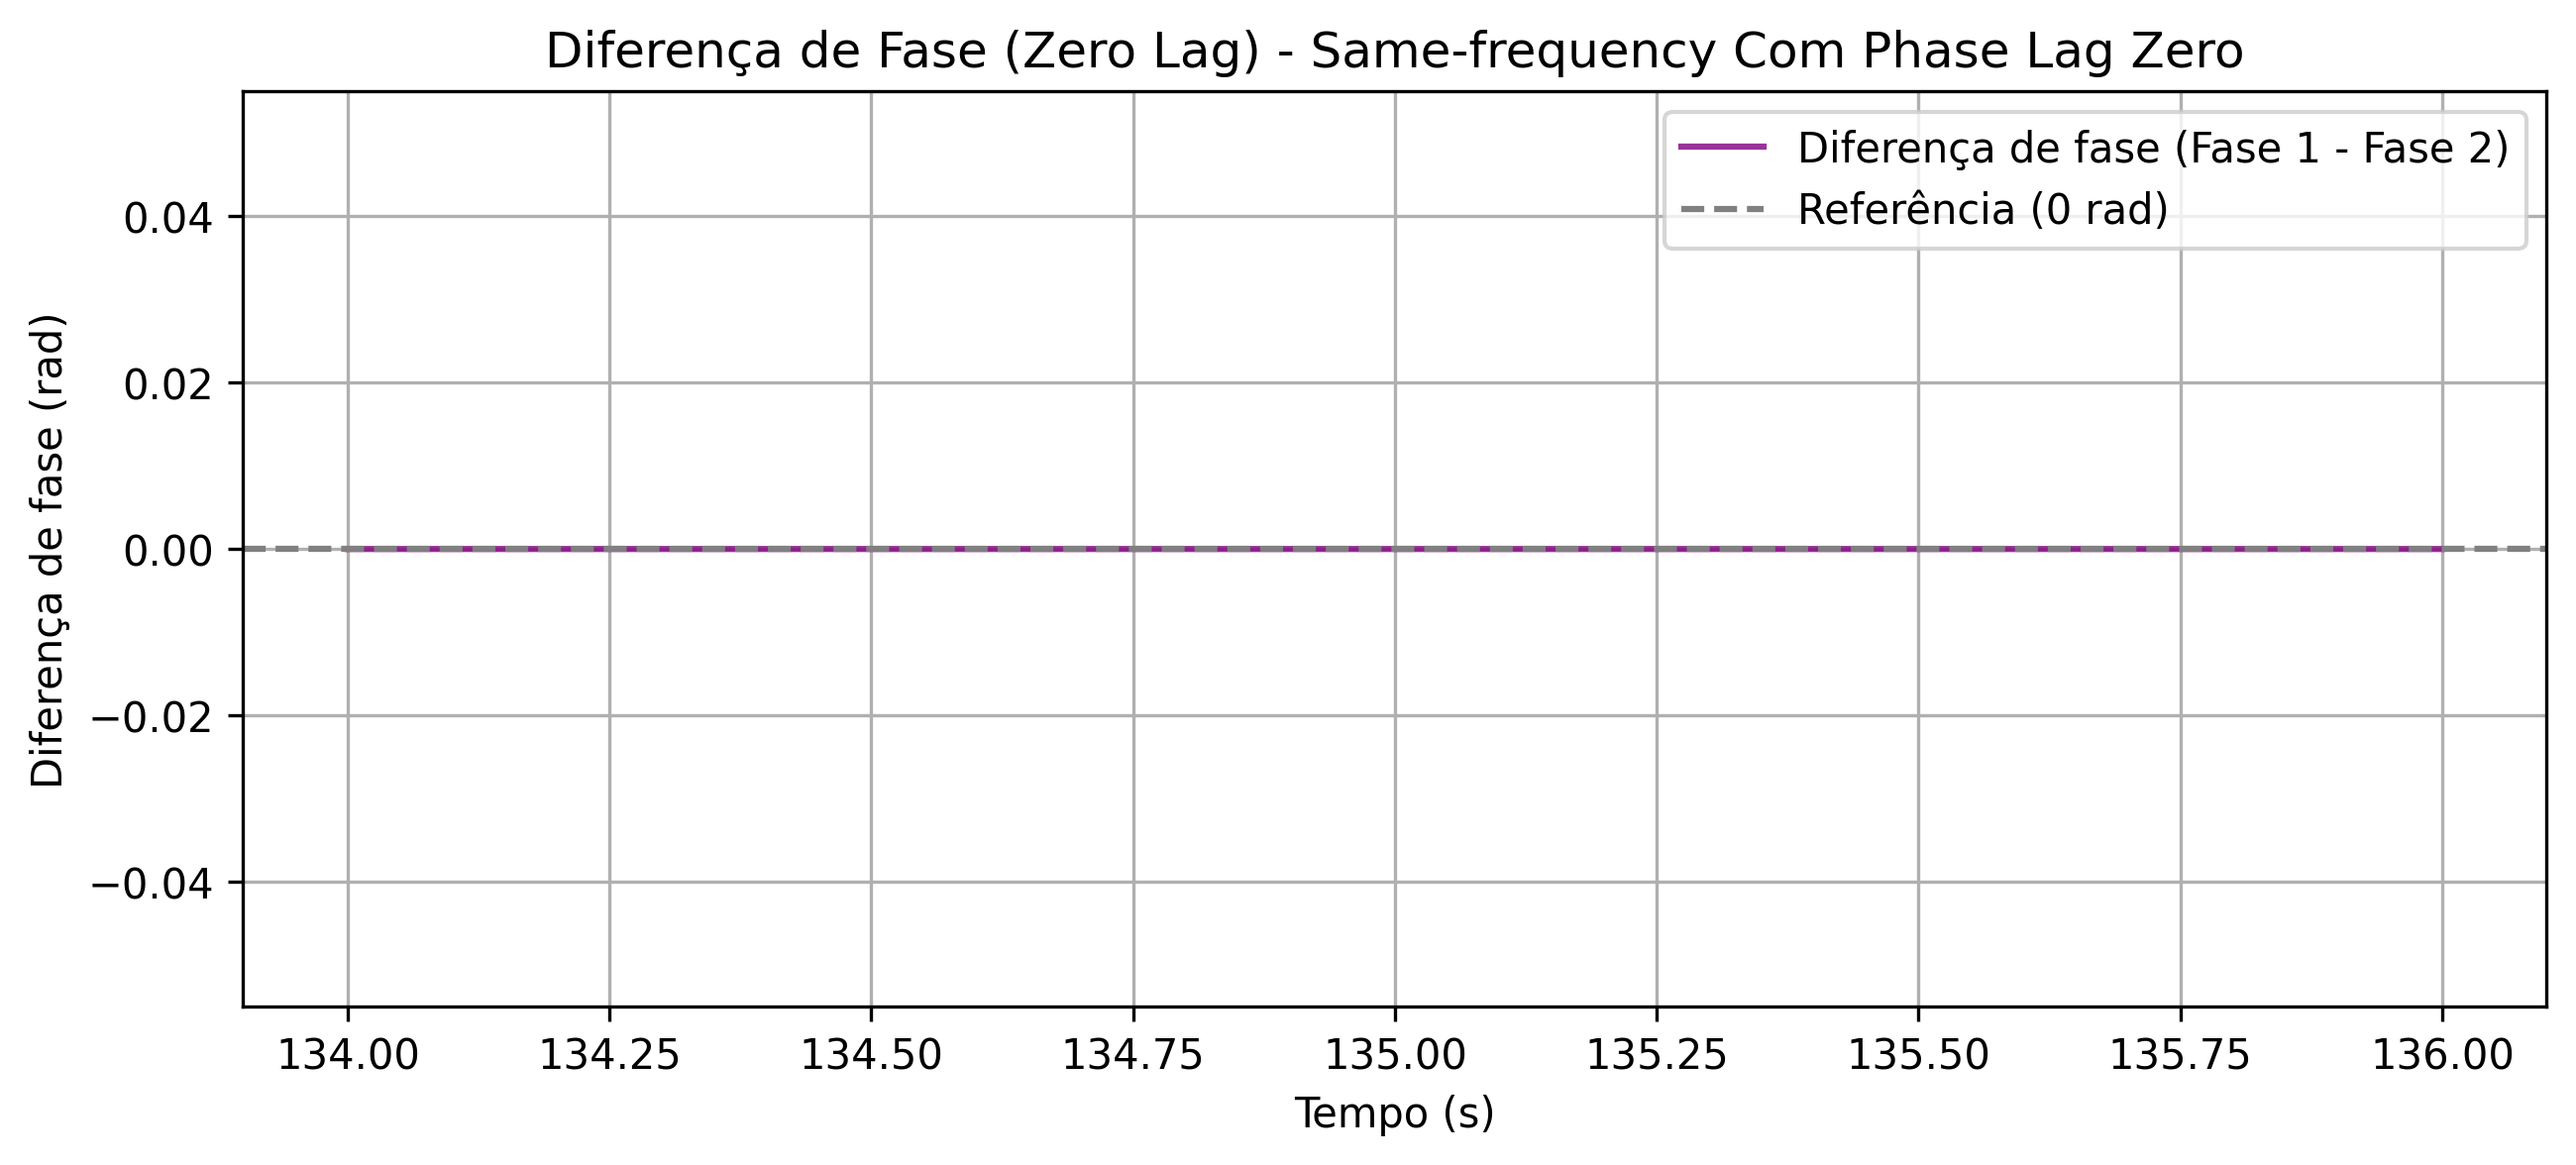
\includegraphics[width=0.8\textwidth]{figs/3_2_testing_connectivity_metrics/16_ZeroLag_Diferenca_Fase_Same-frequency Com Phase Lag Zero.png}
    \caption{Diferença de fase próxima a zero, indicando ausência completa de defasagem no cenário de Phase Lag Zero.}
    \label{fig:zerolag_difference_final}
\end{figure}

O comportamento geral das métricas nos diferentes cenários e níveis de injeção está resumido na Figura~\ref{fig:comparativo_metricas}.

\begin{figure}[htb]
    \centering
    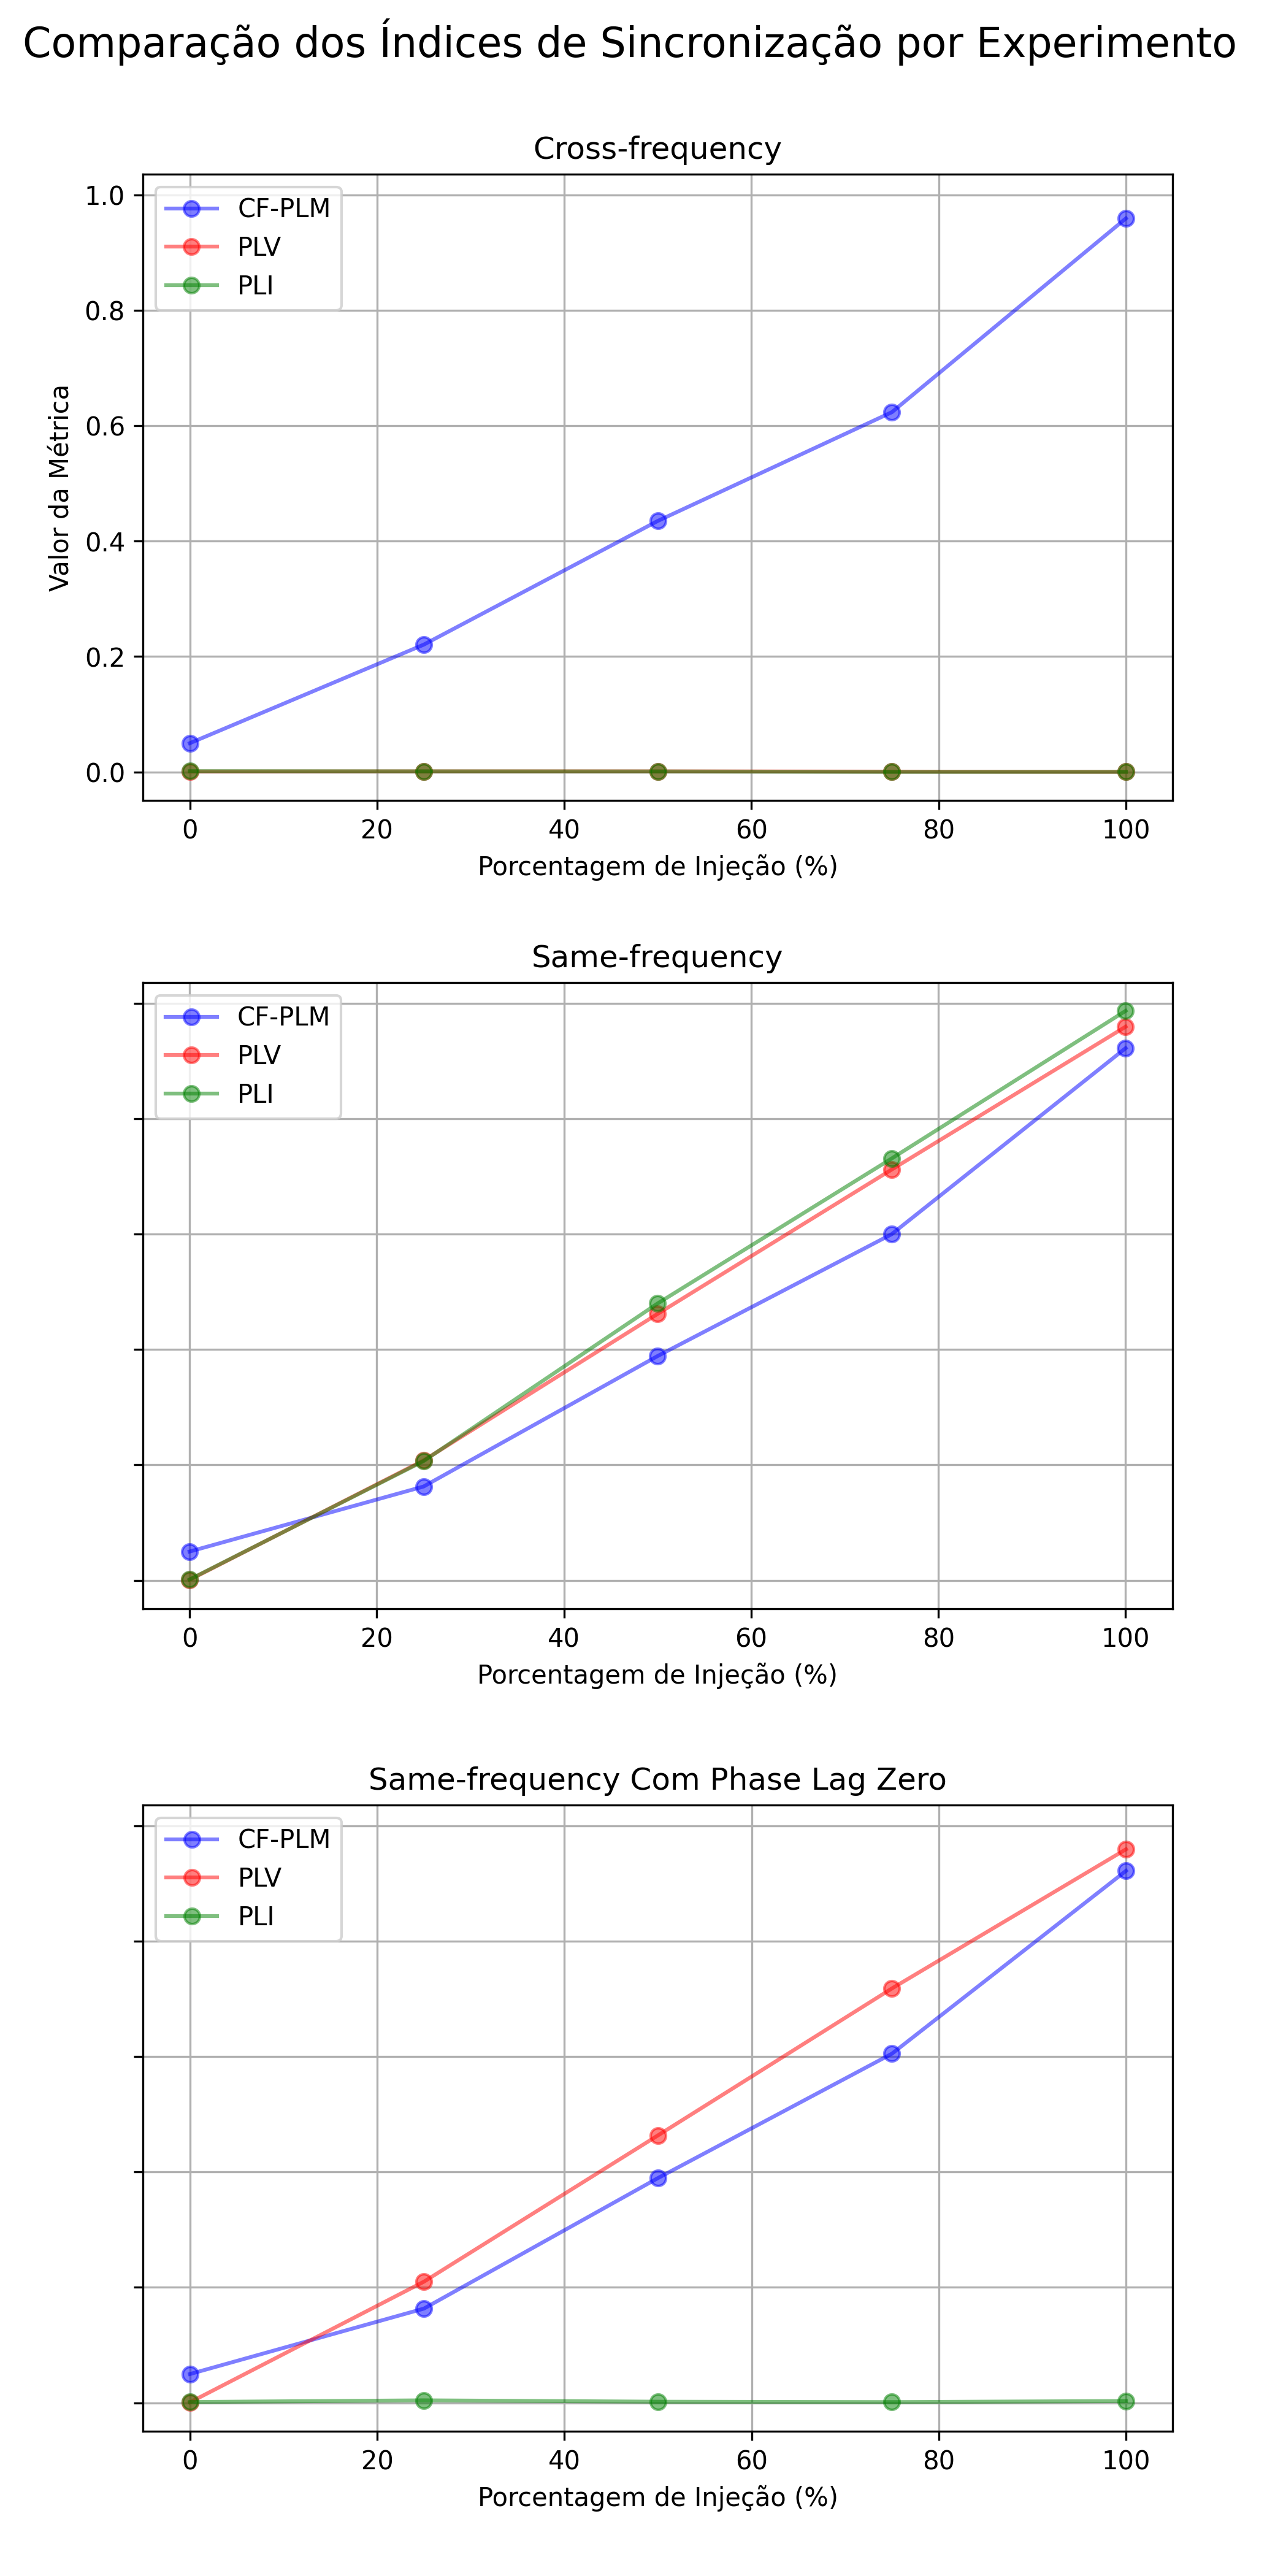
\includegraphics[width=\textwidth]{figs/3_2_testing_connectivity_metrics/17_Comparativo_Subplots_Experimentos.png}
    \caption{Comparação dos índices CF-PLM, PLV e PLI nos três cenários estudados, em função da porcentagem de injeção aplicada.}
    \label{fig:comparativo_metricas}
\end{figure}

Esses resultados justificam a escolha do CF-PLM para análise de sincronização entre ECG e EEG (cross-frequency) e do PLI para sincronização em frequências iguais, evitando detecção de acoplamentos triviais como em condução de volume (phase lag zero). O PLV é reportado apenas para referência complementar devido à sua sensibilidade elevada em condições triviais.

\section{Análise de Conectividade ao Longo do Tempo}
\label{sec:connectivity_over_time}

Para investigar a dinâmica da sincronização ao longo da sessão experimental, o sinal foi dividido em janelas de 10 segundos, ao longo da gravação total de 4 minutos e 30 segundos de cada coleta. Em cada janela, foi calculada uma medida de sincronicidade (PLI, PLV ou CF-PLM) para cada par de canais, para cada banda de frequência, para cada condição (cathodic e sham) e para cada atleta. Em seguida, a mediana desses valores foi extraída, fornecendo uma medida robusta da conectividade ao longo do tempo para cada configuração.

Essa abordagem permite visualizar a evolução temporal da sincronização e comparar a estabilidade dos diferentes índices. Ressalta-se que, em nossas análises, enfatizamos o \emph{Wilcoxon RBC} e o p-valor corrigido por Bonferroni como os principais indicadores de tamanho de efeito e significância estatística, respectivamente, dada sua robustez em contextos não paramétricos e na presença de variabilidade e outliers.

A seguir, são apresentadas as séries temporais obtidas para três métricas principais:
\begin{itemize}
    \item \textbf{CF-PLM (EEG-ECG):} A Figura~\ref{fig:cfplm_time_cat} mostra a mediana do CF-PLM ao longo do tempo para a condição cathodic, refletindo a sincronização cross-frequency entre EEG e ECG.
    \item \textbf{PLI (EEG-EEG):} A Figura~\ref{fig:pli_time_cat} apresenta a mediana do PLI ao longo do tempo para a condição cathodic, indicando a sincronização iso-frequencial entre canais cerebrais.
    \item \textbf{PLV (EEG-EEG):} A Figura~\ref{fig:plv_time_cat} exibe a mediana do PLV ao longo do tempo para a condição cathodic, utilizada aqui para comparação, pois o PLV é mais sensível a ruídos e efeitos de volume conduction.
\end{itemize}

Cada gráfico é construído a partir dos valores calculados em janelas de 10 segundos e a mediana de cada janela foi utilizada para representar a medida de sincronicidade de forma robusta, minimizando o impacto de variações pontuais e outliers.

\begin{figure}[htb]
    \centering
    \includegraphics[width=0.8\textwidth]{figs/4_connectivity_over_time/Mediana_do_CF-PLM_ao_longo_do_tempo_(EEG_ECG)_Catódica.png}
    \caption{Mediana do CF-PLM ao longo do tempo para a condição cathodic (EEG-ECG). Cada ponto representa a mediana da medida de sincronicidade calculada em janelas de 10 segundos, evidenciando a evolução do acoplamento cross-frequency entre EEG e ECG.}
    \label{fig:cfplm_time_cat}
\end{figure}

\begin{figure}[htb]
    \centering
    \includegraphics[width=0.8\textwidth]{figs/4_connectivity_over_time/Mediana_do_PLI_ao_longo_do_tempo_(EEG_EEG)_Catódica.png}
    \caption{Mediana do PLI ao longo do tempo para a condição cathodic (EEG-EEG). O gráfico mostra como a sincronização iso-frequencial entre canais cerebrais varia ao longo da gravação.}
    \label{fig:pli_time_cat}
\end{figure}

\begin{figure}[htb]
    \centering
    \includegraphics[width=0.8\textwidth]{figs/4_connectivity_over_time/Mediana_do_PLV_ao_longo_do_tempo_(EEG_EEG)_Catódica.png}
    \caption{Mediana do PLV ao longo do tempo para a condição cathodic (EEG-EEG). Este índice serve para comparação com o PLI, embora seja mais sensível a ruídos e efeitos de volume conduction.}
    \label{fig:plv_time_cat}
\end{figure}
